%% android.tex
%% by Simon Danner

% The Computer Society requires 12pt.
\documentclass[12pt,journal,compsoc]{IEEEtran}
\usepackage[ngerman]{babel}   
\usepackage[utf8]{inputenc}   % UTF8-Kodierung für Umlaute
\usepackage{hyperref}         % Hyperlinks
\usepackage{listings}
\usepackage{graphicx}

\clubpenalty = 10000           % Keine "Schusterjungen"
\widowpenalty = 10000          % Keine "Hurenkinder"

\selectlanguage{ngerman}

\newcommand{\Monat}{%
\ifcase\month
 Monat 0 \or Januar \or Februar \or März  \or April\or Mai\or Juni\or Juli\or August\or 
 September\or Oktober\or November\or Dezember
\fi}


\newcommand{\paperTitle}{
	Connecting Android powered devices to the external world	
}

\newcommand{\paperSubTitle}{
}

\newcommand{\absatz}{
	\parskip 12pt
}

\newcommand{\paperAuthor}{Simon~Danner}

\newcommand{\todo}[1]{
    \textbf{Todo:}#1
}


% korrigiere Silbentrennung % Kann man auch dazu verwendet die Silbentrennung zu deaktivieren
\hyphenation{op-tical net-works semi-conduc-tor}
% Silbentrennung für ein einzelnes Wort deaktivieren geht mit:
% \mbox{wort}


% Bei einem zwei Spalten Layout versucht Latex auf beide Seiten die gleiche Texthöhe hinzubekommen
% Dies verursacht leider manchmal Leeräume z. B. zwischen der Überschrift und dem Text
% Mit der Option \raggedbottom kann dies unterbunden werdne
% Hat aber den Nachteil das das Dokument so einen unregelmäßigen Seitenfuß hat
% Aber immer noch besser wie die Leerräume
%\raggedbottom

\begin{document}

\title{\paperTitle \\ \paperSubTitle }
\author{\paperAuthor,~\IEEEmembership{ AI7 }}% <-this % stops a space

% The paper headers
% \markboth{Journal of \LaTeX\ Class Files,~Vol.~6, No.~1, January~2007}
% {Shell \MakeLowercase{\textit{et al.}}: Bare Advanced Demo of IEEEtran.cls for Journals}

\IEEEtitleabstractindextext{%
	\begin{abstract}
		TODO Abstract

	\end{abstract}

	% Note that keywords are not normally used for peerreview papers.
	\begin{IEEEkeywords}
		Android, Hardware, Arduino, IOIO ADK, ADK 2012, AOA, Bluetooth LE  
	\end{IEEEkeywords}
}

\maketitle

\section{Einleitung}


\IEEEPARstart{A}{}ndroid ist mit einem Marktanteil von ca. 85\% nach IDC das zur Zeit am weitesten verbreitete Smartphone und Tablet Betriebssystem.\cite{marketshare}
Android wird auf Smartphones, Tablets, Smartwatches, Fernsehern und anderen Geräten verwendet.
Da die Nutzer solcher Geräte, diese oft rund um die Uhr bei sich tragen, bietet es sich an, diese Geräte zur Steuerung von anderen elektronischen Geräten zu nutzen.





% Datum
\hfill{\the\day~\Monat, \the\year  }

\section{Allgemeines}
TODO Nutzen, Entwicklung

\section{Anbindungsmöglichkeiten}
Mittlerweile gibt es mehrere Möglichkeiten, Hardware mit Android Geräten zu verbinden. 
Diese decken ein großes Spektrum an Anwendungsmöglichkeiten ab, wobei jede Vorteile und Nachteile bei bestimmten Anwendungen besitzt.
Nach ersten experimentellen Ansätzen von Hobbyentwicklern und einzelnen Firmen, hat auch Google den Nutzen einfacher Verbindung mit externen Geräten 
erkannt und bietet seit 2011 offiziell unterstützte Möglichkeiten, dies zu realisieren. 

\section{ADB (Android Debug Bridge)}
\subsection{Grundlagen}
Die Android Debug Bridge ist eine Softwaresuite mit der es möglich ist, von Host PCs mit Android Geräten zu kommunizieren.
Der Hauptnutzen besteht darin, Android Applikationen in einem virtuellen Gerät (Emulator) oder direkt auf echten Geräten zu debuggen.
Dabei wird auf dem Host ein Server gestartet, welcher die Kommunikation zwischen Host und Endgerät übernimmt. 
Die Clients (z.B. dem adb command line tool, oder IDEs wie Android Studio), verbinden sich mit dem Server und senden Befehle an das über USB (oder Wifi) mit dem Server verbundene Endgerät.
Auf den Endgeräten oder im Emulator läuft im Hintergrund ein Dienst, der die Kommandos vom Server entgegennimmt und antwortet. Die Kommunikation mit dem Server läuft über TCP,
was es Clients ermöglicht sich über das Netzwerk mit Servern zu verbinden. (Siehe Abbildung \ref{adb})
Der ADB Dienst auf den Endgeräten muss explizit durch den Nutzer aktiviert werden, bevor er benutzt werden kann.
Da adb für das debuggen von Apps, also für Softwareentwickler konzipiert ist, stellt dies im allgemeinen kein Usability Problem dar.

\begin{figure}
	\centering
	\caption{Android Debug Bridge Architektur}
	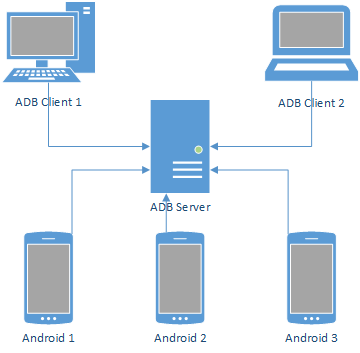
\includegraphics[width=0.4\textwidth]{media/adb.png}	
	\label{adb}
\end{figure}

\subsection{Verwendung mit externen Geräten}
Außer dem benutzten der ADB zum debuggen, kann die Architektur auch benutzt werden, um eigene Kommunikationsprotokolle zu implementieren.
Dabei wird das eigene Protokoll als eine Zusatzschicht über adb, in Form von Kommandos implementiert. TODO ??


TODO wann von wem zur Device kommunikation ?? --> IOIO


\section{AOA (Android OpenAccessory)}
Android OpenAccessory ist der Name eines von Google entwickelten Protokols, was 
dezidiert für die Anbindung von externen Geräten an Android Geräte entwickelt wurde.
Die erste Version (ADK 2011) wurde im Mai 2011 vorgestellt.
Das ADK besteht aus einer Hardware Referenz Platform, sowie Source Code für diese, damit 
Entwickler einfach Hardware und Software anpassen und erweitern können.
\cite{developaoa}
\subsection{Ziel}
Ziel Googles ist es mithilfe des AOA einen einheitlichen Standard zur Verbindung von externen Geräten mit Android Geräten zu etablieren.
Dies führt dazu, dass Endanwender ohne auf spezille Gerät Kombinationen verwendet zu müssen, externe Hardware kaufen und benutzen können.
Google veröffentlichte bisher (Stand September 2014), zwei Versionen des ADKs, 2011 und 2012. 

\subsection{ADK 2011}
Beim ADK 2011 wurde von Google eine
Referenzplatform auf Basis eines Arduino Mega 2560, welcher ein USB Host TODO enthält, sowie eine Arduino Bibliothek zur Kommunikation mit fähigen Android Geräten veröffentlicht.
Die Android seitige Funktionalität des AOA wurde in Android 2.3.4 (Release April 2011) und spätere Versionen integriert. 

TODO Protokoll
TODO Beispiele
\subsection{ADK 2012}
\subsubsection{Änderungen}

\subsubsection{Audio}
Android unterstützt Entwickler beim einbinden von Audio Geräten. Das Verwalten der Hardware wird von Android komplett übernommen.
Enwickler von Audio Applikationen können optional über den AudioManager herausfinden, was für Geräte angeschlossen sind. So kann man zum Beispiel die Lautstärke anpassen wenn ein Bluetooth Headset verbunden wird, oder Kopfhörer entfernt werden.
Da die Verwendung von Audio Geräten fast automatisch abläuft, wird hier nicht weiter auf Audio Geräte eingegangen.
Historisch gab es einige Entwicklungen die Audioausgabe zur Übermittlung an externe Geräte zu verwenden. Diese sind jedoch in Anbetracht heutiger Möglichkeiten eher als historische Kuriositäten von Bastlern zu sehen.
Ein Beispiel für ein solches Projekt ist Project HiJack \cite{hijack} , welches eine Hard- und Software Platform zur Übermittlung von Signalen und Verarbeitung dieser auf Microcontrolern unter iOS sowie Android entwickelte.
Die Probleme hierbei sind vor allem die analoge Übertragung und die relativ begrenzte Bandbreite.
\section{Bluetooth}
\subsection{Bluetooth Low Energy}
Bluetooth Low Energy, kurz BLE ist seid 2009 optionaler Teil des Bluetooth Standard Version 4.0. 
Ziel von BLE ist es, den Stromverbrauch mittels darauf optimierter Protokolle und anderer Einschränkungen gegenüber Bluetooth zu veringern.
In Smartphones wurde BLE in nennenswertem Umfang zuerst von Apple mit iOS 5 ( Oktober 2011)unterstützt.
Von Android wird Bluetooth LE ab der Version 4.3 (Release Juli 2013) unterstützt.
BLE ermöglicht es Chips zu entwickeln, die nur dieses Protokoll unterstützen (kein volles Bluetooth TODO), was die Chips für Hardwarehersteller billiger und einfacher zu verwenden macht.
TODO Geschichte
TODO Nutzen
TODO Implementierung / Code ??


\subsection{NFC TODO}




\section{Beispiel AOA}
\subsection{Vorhaben}

\subsection{Umsetzung}

\subsection{Erkenntnisse}


\section{Ausblick}
Zukunft TODO
\subsection{AOA}

\subsection{Bluetooth}
\subsection{andere Techniken}

\section{Fazit}






\bibliographystyle{IEEEtran}
\bibliography{android_quotes}

\end{document}

